\begin{figure}[tbp]
        \centering
        \resizebox{0.6\linewidth}{!}{%
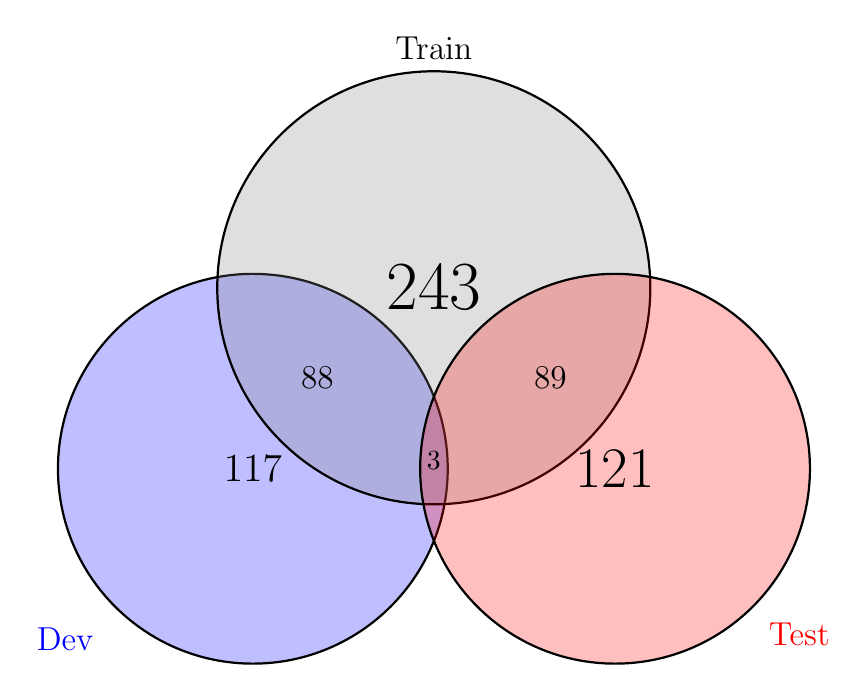
\begin{tikzpicture}[ 
    set/.style = {draw, circle,
        minimum size = 4.95cm}]
  
\node (A) [
    set,
    fill = blue,
    fill opacity = 0.25,
    text opacity = 1,
    label = {[label distance=0.2cm,blue]225:\large Dev},
    thick
    ] {\Large  \textbf{$117$}};
\node (B) at (45:3.25cm) [
    set,
    minimum size = 5.5cm,
    fill = gray,
    fill opacity = 0.25,
    text opacity = 1,
    label={[label distance=0.01cm]90:\large Train},
    thick
    ] {\Huge \bf $243$};
\node (C) at (0:4.6cm) [
    set,    
    fill = red,
    fill opacity = 0.25,
    text opacity = 1,
    label={[label distance=0.1cm,red]315:\large Test},
    thick
    ] {\huge $121$};
 
\node at (barycentric cs:A=1,B=1) [left] {\large $88$};
%\node at (barycentric cs:A=1,C=1) [below] {0};
\node at (barycentric cs:B=1,C=1) [right] {\large $89$};
\node at (barycentric cs:A=1,B=0.1,C=1) [] {3};
\end{tikzpicture}%
}
        \caption{\small Number of signers per train, dev, and test corpus of~\cite{moryossef_realtime_2020}. Numbers in the overlapping regions indicate signer overlaps between the sets. \vspace{-4mm}}
        \label{fig:datasets_dgsoriginal_overlap}
    \end{figure}